% master file siminos/froehlich/slice/slice.tex
% $Author$ $Date$

% \section{\Mslices}
%       \label{sec:mslices}

Suppose you are observing turbulence in a pipe flow, or your
defibrillator has a mesh of sensors measuring electrical currents that
cross your heart, or you have a precomputed pattern, and are sifting
through the data set of observed patterns for something like it. Here you see a
pattern, and there you see a pattern that seems much like the first one.
How ``much like the first one?''
Think of the first pattern (represented
by a point {\slicep} in the \statesp\  \pS) as a
`template'\rf{rowley_reconstruction_2000,rowley_reduction_2003} or a
`reference state' and use the symmetries of the flow to slide and rotate
the `template' until it overlays the second pattern
(a point $\ssp$ in the \statesp), \ie, act with elements of
the symmetry group \Group\ on the template ${\slicep} \to
{\LieEl}{\slicep}$ until the distance between the two patterns
\beq
|\ssp - {\LieEl}{\slicep}|
    = |\sspRed - \slicep|
    \label{minDistance0}
\eeq
is minimized. Here $\sspRed$ is the point on the group orbit
of $\ssp$,
\beq
\ssp=\LieEl \sspRed
	\qquad
\LieEl \in \Group
\,,
\ee{sspOrbit}
closest to the template {\slicep}, where we shall measure distance
$|\ssp|^2=\braket{\ssp}{\ssp}$ in terms of the Euclidian inner product
\( %beq
\braket{x}{y} = \sum_i^d {x}_i y_i
%    \,,\; %\qquad
% x, y \in \pS \subset \reals^d
	\,,
\) %\ee{innerR}
or, if the \statesp\ is a normed function space,
\( %\beq
\braket{g}{f} = \int dx \, \dual{g}(x) f(x)
\,,
\) %\ee{innerL2}
with the associated $L^2$ norm $|f|^2 = \braket{f}{f}$.
In practice, we always represent such functions by discrete
meshes or truncated basis sets, with a (possibly large)
finite-dimensional \statesp\  $\pS \subset \reals^d$.

If we parameterize a Lie group element $\LieEl=\LieEl(\gSpace)$ by
parameters $\gSpace = (\gSpace_1,\gSpace_2,\cdots\gSpace_N)$, the minimal
distance satisfies the extremum conditions
\beq
0  =
\frac{\partial ~~}{\partial \gSpace_a} |\ssp - \LieEl\slicep|^2
   =
\braket{\sspRed - \slicep}{\sliceTan{a}}
    \,,\qquad
	  \sliceTan{a} = \Lg_a \slicep
\,.
\label{PCsectQ}
\eeq

More explicitly, an element of a compact Lie group that is continuously
connected to the identity can be expressed as
\beq
\LieEl(\gSpace)=e^{{\gSpace} \cdot \Lg }
    \,,\qquad
\gSpace \cdot \Lg = \sum_{a=1}^N \gSpace_a \Lg_a
\,.
\ee{FiniteRot}
The group action parameters $\gSpace_a$ are often referred to as
``phases,'' or ``shifts.''
The group orbit of a point $\ssp$ under the group $\Group$ is the set of all
points that $\ssp$ is mapped to under the groups actions
\beq
\pS_\ssp=\{{g} \, \ssp: g \in \Group\}.
\ee{GroupOrbit}
As \Group\ is a symmetry of the system, the
length $|\ssp|$ is invariant under symmetry operations, $\Group \subset \On{d}$
and the Lie algebra {generators} $\Lg_a$ are a set of $N$ linearly
independent $[d\!\times\!d]$ antisymmetric matrices acting linearly on
the {\statesp} vectors $\ssp \in \pS \subset \reals^d$. An infinitesimal
% , $|\delta \gSpace| \ll 1$,
group action is generated by
$
\LieEl(\delta \gSpace) \simeq 1 + \delta \gSpace \cdot \Lg
\,.
$ %\ee{eq:infinitesimal}
A transformation induced by an infinitesimal
time-dependent variation of group `phases'
$\delta \gSpace_a = \timeStep \, \dot{\gSpace_a}$ is
\beq
\dot{\ssp} = \dot{\gSpace} \cdot \groupTan(\ssp)
\,,
\ee{PC:groupTan1}
where
\beq
 \groupTan_{a}(\ssp) = \Lg _{a} \ssp
    \,,\qquad
 a=1,2,\cdots,N,
\ee{PC:groupTan}
is the group action tangent at $\ssp$.
So $\dot{\gSpace} \cdot \groupTan(\ssp)$ is the velocity
of the flow along the group orbit of \ssp.
We use $\groupTan_a(\ssp)$ notation (rather than
$\Lg_{a}\ssp$) to emphasize that the group action
induces a \emph{tangent field} at $\sspRed$.


{\bf Slice:}
The minimum distance condition \refeq{minDistance0} together with
Euclidean norm says that the
closest point $\sspRed$ in the group orbit of \statesp\ point $\ssp$ lies in a
$(d\!-\!N)$-dimensional hyperplane defined by \refeq{PCsectQ},
a hyperplane through the template point $\slicep$,
normal to the group action tangent
space $\sliceTan{}$.
This hyperplane is called a `slice' and is an example of
symmetry reduction by transverse sections of
group orbits\rf{FelsOlver98,FelsOlver99,OlverInv} that
can be traced back to Cartan's \mframes\rf{CartanMF}.

As a generic group orbit is a curved $N$-dimensional manifold embedded in
the \statesp, several values of $\gSpace$ might be local extrema of the
distance function \refeq{PCsectQ}. For example, group orbits of \SOn{2}\
are topologically circles, and the distance function \refeq{minDistance0}
has maxima, minima and inflection points as extrema. We only care about
those that are local {\em minima}, for which all the eigenvalues of the
symmetric matrix $[N\!\times\!N]$ matrix of second derivatives of
distance,
\beq
\frac{\partial^2}
     {\partial \gSpace_a \partial \gSpace_b}
        |\sspRed - \slicep|^2
    =
%  - \braket{\Lg_a e^{\gSpace \cdot \Lg} \ssp}{\sliceTan{b}}=
  - \braket{\groupTan_a(\sspRed)}{\sliceTan{b}}=
  \braket{\sspRed}{\Lg_a \Lg_b\slicep}
\ee{PCinflPoint}
are positive.

$\Lg_a \Lg_b$ plays a fundamental role in the theory of Lie groups.
Any representation of a compact group $\Group$ is fully
reducible, and for a Lie group
the invariant tensors constructed by contractions
of $\Lg_a$ are useful for identifying irreducible
representations. The simplest such invariant is
\beq
\dual{\Lg} \cdot \Lg = \sum_\alpha C_2^{(\alpha)} \, \id^{(\alpha)}
\,,
\ee{QuadCasimir}
where $C_2^{(\alpha)}$ is the quadratic Casimir for
irreducible representation labeled $\alpha$, and
$\id^{(\alpha)}$ is the identity on the $\alpha$-irreducible
subspace, 0 elsewhere. $ C_2^{(\alpha)} =0$ if $\alpha$
is an invariant subspace.
The dot product of two tangent fields in
\refeq{PCinflPoint} is thus a sum of inner products
weighted by Casimirs,
\beq
\braket{\groupTan(\sspRed)}{\groupTan(\slicep)}
   = \sum_\alpha C_2^{(\alpha)} \dual{\sspRed}_i\, \delta_{ij}^{(\alpha)} \slicep_j
\,.
\ee{braket}
An example is the Fourier series \refeq{tangL2norm}.
For compact groups $C_2^{(\alpha)}$ are strictly nonnegative by
the antihermiticity \refeq{antiHerm} of Lie algebra generators.


The physically most interesting minimum is
presumably the closest one, the absolute minimum of \refeq{minDistance0}.
It does not matter whether the group is compact, for example $\SOn{n}$, or
noncompact, for example the Euclidean group $E_2$ that underlies the generation
of spiral patterns\rf{Barkley94}; in either case any group orbit has
one or several locally closest passages to the template state.







If the two patterns are
close, their group orbits will be nearly parallel, and for a smooth flow
the slice will be transverse to all group orbits of $\ssp$ in a
neighborhood of \slicep.

%    \PC{recycle this:
%{\em {\mslices}}
%    }


By the antihermiticity of $\Lg$, \refeq{antiHerm},  we have
$\braket{\slicep}{\sliceTan{a}}=0$, and the transformation parameters
$\gSpace$ for which the state $\ssp$ is closest to the template
$\slicep$ are fixed by $N$ slice conditions
\beq
\braket{\sspRed}{\sliceTan{a}} =0
    \,,\qquad
\sspRed = \LieEl(\gSpace) \ssp
\,.
\ee{PCsectQ0}

A given compact group orbit intersects a slice at least twice, and
possibly many times, so we need a prescription for how to
pick a unique \reducedsp\ point as the representative of the entire group
orbit.


However, we will be bolder, and show next that for a generic template
$\slicep$ (\ie, any $\slicep$ whose group orbit is $N$-dimensional), the
slice hyperplane \refeq{PCsectQ} cuts across the group orbit of {\em
every} point in the full \statesp\ \pS.





The distance surface $|\sspRed - \slicep|$ can have inflection points,
What role do they play? They are non-generic, but if we consider distance
to local minima at successive instants of a time-evolving trajectory,
coalescence of
nearby minima, maxima pairs cannot be avoided. At the instant of
coalescence the denominator in \refeq{SF:sliceEas} goes through a simple
pole, and the integrated trajectory within slice might jump.



\subsection{}
\subsubsection{}


\section{Dynamics in the slice}
\label{sect:MovFrameODE}

The \reducedsp\ trajectory is given by $\ssp(\tau)=\LieEl(\tau)
\sspRed(\tau)$. Differentiating both sides with respect to time and
setting $\velRed={d\sspRed}/{d\tau}$ we find
\[
\vel(\ssp)=\dot{\LieEl} \, \sspRed+\LieEl \, \velRed(\sspRed) \]
\[
\vel(\LieEl \, \sspRed)=\dot{\LieEl} \, \sspRed+\LieEl \, \velRed(\sspRed) \]
\[
\vel=\velRed + \LieEl^{-1} \, \dot{\LieEl} \, \sspRed
\,.
\]
The product of the inverse of the Lie group element and its time
derivative give the group tangent at the point:
$\LieEl^{-1}\dot{\LieEl}=e^{-\gSpace \cdot \Lg} \,
\frac{d ~~}{d \, \tau} e^{\gSpace \cdot \Lg}=\dot{\gSpace}\cdot \Lg$,
leaving us with the equation for the velocity of the reduced flow in the slice:
\beq
\velRed(\sspRed)=\vel(\sspRed)-\dot{\gSpace}(\sspRed)\cdot \groupTan(\sspRed).
\ee{eq:redVel}
This says that the velocity in the full \statesp\ is the sum of the
velocity in the slice and the velocity normal to it, along the group
tangent.

This equation is true for any factorization $\ssp(\tau)=\LieEl(\tau)
\sspRed(\tau)$, and by itself provides no information on how to calculate
$\dot{\gSpace}$. Let
$\sliceTan{a}$ be the group tangents at the slice
fixing point. When require that the flow stays in the slice,
as in \refeq{PCsectQ0},
we find that $\gSpace$ must satisfy the system of equations:
\beq
\braket{\vel(\sspRed)}{\sliceTan{a}}
 -\braket{\dot{\gSpace}\cdot \groupTan(\sspRed)}{\sliceTan{a}}=0
\,.
\label{eq:slicecondition}
\eeq
% for each group tangent $\sliceTan{a}$ at the slice fixing point.
In principle this is a matrix equation one can solve
for $\dot{\gSpace}_a$.
$\SOn{2}$ is the easiest case, as it has a single group tangent,
resulting in the explicit system of equations:
\bea
\dot{\gSpace}(\sspRed) &=& \frac{\braket{\vel(\sspRed)}{\sliceTan{}}}
               {\braket{\groupTan(\sspRed)}{\sliceTan{}}}
\continue
\velRed(\sspRed) &=& \vel(\sspRed)
   -\dot{\gSpace}(\sspRed) \groupTan(\sspRed).
\label{eq:so2reduced}
\eea

 \begin{figure}
 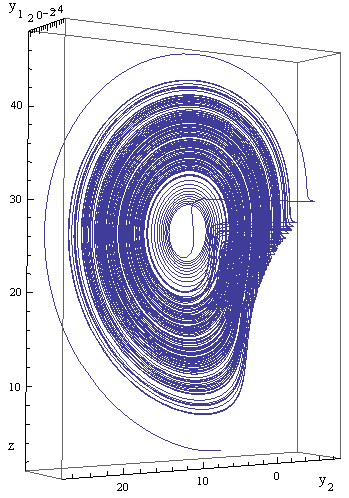
\includegraphics[width=0.35\textwidth]{CLEreduced}%
 \caption{\label{fig:CLErx2y1z}
A $\{y_1,y_2,z\}$ plot of the \reducedsp\ \cLf\ strange attractor
with initial point
%$(x_1, x_2, y_1, y_2, z) = (1, 2, 3, 1, 2)$
in the
slice normal to $\sliceTan{}=(1,0,0,0,0)$. Contrast this plot with
\reffig{fig:CLEx2y1z}, and note the apparent discontinuities in the
reduced flow.
 }%
 \end{figure}

\subsection{Traversing a slice singularity}
\label{sect:passingSing}

\beq
\braket{\groupTan(\sspRed)}{\sliceTan{}}=0
\ee{sliceSingl}

 \begin{figure}
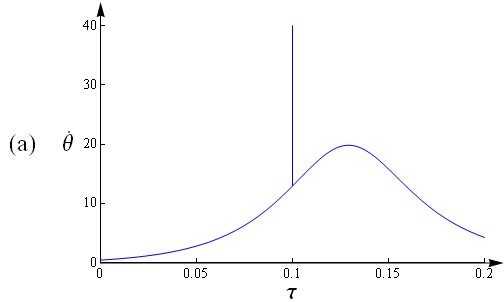
\includegraphics[width=0.45\textwidth]{CLEsingpass}
\\
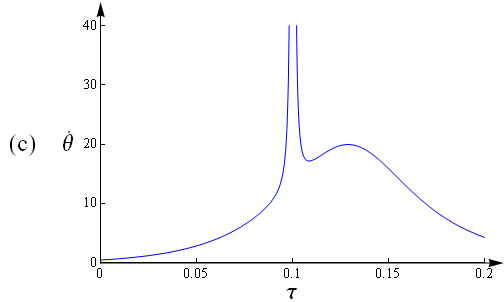
\includegraphics[width=0.45\textwidth]{CLEnearsing2}%
 \caption{\label{fig:dthetasing}
The group velocity $\dot{\gSpace}$ for two \CLf\
\reducedsp\ trajectories in a slice defined by the slice-fixing
point $\slicep=(0.782?,-0.277?,-0.4?,0.12?,0)$:
 (a) As trajectory $\sspRed(\tau)$ passes through the singularity
\refeq{sliceSingl}
%$\braket{\groupTan(\sspRed)}{\sliceTan{}}=0$
 at $\sspRed=(-1.22?, ?3.212, -?4.31, ?1.11, ?4)$,
the group velocity diverges
$\dot{\gSpace} \to \infty$ as a Dirac delta function.
(b) The group velocity for a nearby trajectory going
through $\sspRed+\delta \sspRed$,
where $\delta\sspRed=(0.01,0,0,0,0)$.
 }%
 \end{figure}

 \begin{figure}
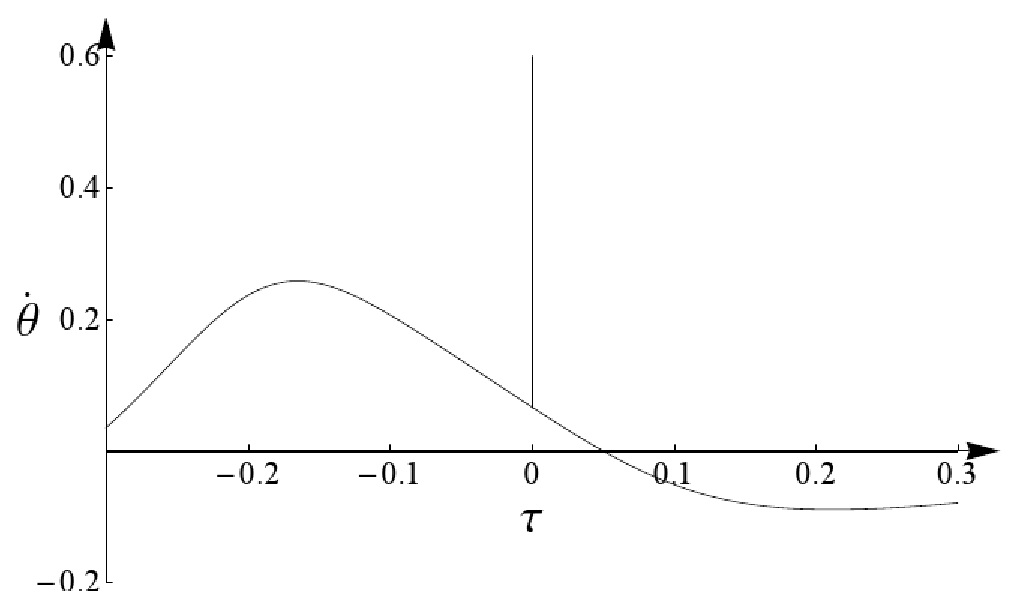
\includegraphics[width=0.45\textwidth]{singpass}
 \caption{\label{fig:singpass}
The blue trajectory passes through the singularity point
$x_{sing}=(-0.44, 3.23, -0.034, 6.37, 2.34)$ in the slice normal to
$(-0.45, -1.05, 0.3, 0.5, 0.)$. Notice how there is the gap in the
trajectory, this corresponds to the jump cause by passing through the
singularity. The red trajectory has initial point differing from the
blue's by $(0,0,0.1,0,0)$, so it does not pass through a singularity. The
green trajectory is the group orbit of $x_{sing}$ between the two
$\gSpace$ that rotate $v(x_{sing})$ in the slice. Notice how, as
predicted, the red trajectory begins near the blue trajectory, closely
follows the green trajectory after the singularity point, reaches the
other side of the blue trajectory and begins to follow it
again.
 }%
 \end{figure}


%
% ****** End of file slice.tex ******
